%%%
 % File:     replay.tex
 % Author:   Hackademics Forum <hackademicsforum6@gmail.com>
 % Project:  MindMap des vulnérabilités
 % Released: 03/08/2016
%%%

%!TeX root = main.tex
%!TeX encoding = UTF-8
%!TeX program = pdflatex
%!TeX spellcheck = fr_FR

%%%
 % Vulnérabilités Replay
%%%
\newpage
\section{Rejeu (Replay / Playback)}\label{vulnerabilites:reseau:replay}

Une attaque par rejeu ou "Replay Attack" est une attaque de type "Man In The Middle". Cette attaque permet à un pirate d'espionner les données échangées entre deux ordinateurs afin de capturer les paquets et d'enregistrer des données utiles et confidentielles d'authentification qui pourront ensuite être réutilisées malgré le chiffrement pour être soumises à un ordinateur (client/serveur) afin être rejoués tel quels, comme par exemple des transactions bancaires. Mais cette technique ne se limite pas aux banques et peut être utilisé pour voler des informations de connexion de boite e-mail, voler votre numéro de carte bancaire ou tout type de données personnelle qui sera utilisé par le/les pirates pour leurs activité illégales. Le rejeu permettra de faire croire en une connexion légitime et pourra permettre au pirate de s'authentifier et avoir accès au système en usurpant l'identité de la victime. 

\begin{flushleft}
Pour capturer les paquets, le hacker pourra utiliser un script fait maison ou alors plus simplement des logiciels comme wireshark, tcpdump ou zed attack proxy. Ces paquets seront généralement enregistrés au format pcap. Il utilisera ensuite soit à nouveau un script fait maison ou alors un logiciel de type tcpreplay pour renvoyer (rejouer) ces paquets afin de se faire passer comme quelqu'un de légitime.
\end{flushleft}

\bigskip

\begin{itemize}
\item Des informations utiles sont envoyées a travers le réseau
\item Un hacker pourra utiliser ces informations afin de les réutiliser a mauvais escient
\item Il aura besoin d'un accès aux données qui se fera
\begin{itemize}
\item Physiquement
\item MITM 
\item Malware
\end{itemize}
\item Les informations récupérées seront utiles au pirate
\item Qui pourra les réutiliser en les rejouant pou paraître comme légitime
\end{itemize}

\bigskip

\begin{flushleft}
\textbf{Exemple}
\end{flushleft}

\smallskip

\begin{flushleft}
Supposons une communication entre deux ordinateurs A et B. A va envoyer sa clef à B pour prouver son identité. Mais un pirate C est en train d'espionner cette conversation et décide de garder les informations ainsi obtenues dans la conversation entre A et B. Ces informations lui seront utiles pour se faire passer comme légitime en rejouant les données de connexion à B
\end{flushleft}

\smallskip

\begin{center}
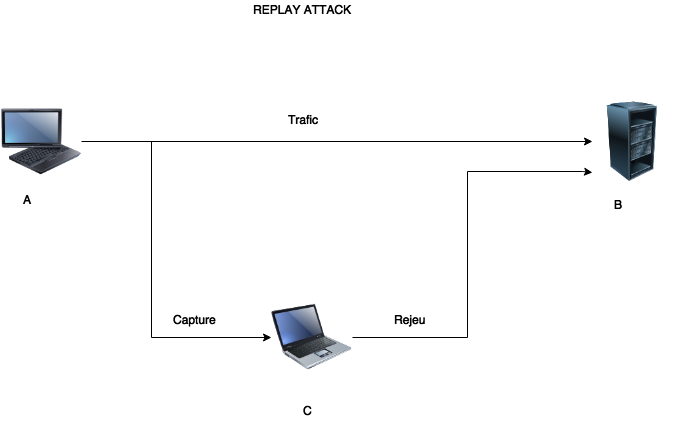
\includegraphics[scale=0.3]{Network/assets/rejeu.png}
\end{center}

\bigskip


\begin{flushleft}
\textbf{Contre-mesures}
\end{flushleft}

\smallskip

\begin{itemize}
\item Le chiffrement n'étant pas suffisant pour contrer les attaques par rejeu il est
conseillé d'utiliser.
\item L'utilisation d'un nombre arbitraire (NONCE) généré aléatoirement a usage
unique qui sera utilisé pour signer les échanges de données. En utilisation avec
un protocole de challenge-réponse.
\item L'utilisation d'horodatage chiffré est un autre moyen d’empêcher les
attaques par rejeu. La synchronisation devrait être réalisée en utilisant un
protocole sécurisé.
\item L'utilisation de mots de passe a utilisation unique qui expirent après un
certain temps.
\item Un numéro de séquence peut être utilisé. L'authenticité de ce numéro pourra
être vérifiée par un code d'authentification de message.
\item l'utilisation de tokens de session unique en utilisant un processus de
génération aléatoire.
\end{itemize}

\bigskip

\begin{flushleft}
\textbf{Exemple}
\end{flushleft}

\smallskip

\begin{flushleft}
Pour prévenir d'une attaque par rejeu on pourrait calculer le delta (différence) entre l'horodatage du client et celui du serveur. Cette différence ne sera pas autorisée a être plus grande que (par exemple) une minute (mais le delta sera autorisé a changer périodiquement pour autoriser les changements horaires). En complement l'utilisation d'un NONCE de grande taille (on pourrait aussi utiliser un NONCE alphabétique ou alphanumérique). L'utilisation de l'horodatage et du NONCE devraient être protégés par l'implémentation d'un  HMAC (Algorithme Hash-based Message  Authentication Code).
\end{flushleft}

\bigskip

\begin{flushleft}
\textbf{Lien-utiles}
\end{flushleft}

\begin{itemize}
\item \url{https://www.owasp.org/index.php/Testing_for_WS_Replay_(OWASP-WS-007)}
\item \url{https://www.sitepoint.com/how-to-prevent-replay-attacks-on-your-website/}
\item \url{item h222767.temppublish.com/15_NS/NS_lecture9.ppt}
\item \url{https://tools.ietf.org/html/rfc2085}
\item \url{https://tools.ietf.org/html/rfc2289}
\item \url{https://tools.ietf.org/html/rfc7384}
\end{itemize}

\endinput
